\documentclass{article}

\usepackage{xeCJK}
\usepackage{ctex}

\usepackage{geometry}
\geometry{left=1.25in,right=1.25in,top=1in,bottom=1in}

\usepackage{fancyhdr}
\pagestyle{fancy}
\lhead{ACM-ICPC模板整理}
\rhead{UESTC\_Continue}

\usepackage{fontspec}
\newfontfamily\mono{OperatorMono-Book}
\newfontfamily\boldmono{OperatorMono-Bold}

\usepackage{listings}
\lstset{
  basicstyle=\linespread{1}\small\mono,
  keywordstyle=\boldmono,
  commentstyle=\itshape,
  frame=single,
  language=[11]C++,
  morekeywords={size_t, uintmax_t},
  tabsize=2,
  showstringspaces=false,
}

\usepackage{amsmath, amssymb}
\usepackage{relsize}

\usepackage{booktabs}
\usepackage{array}
\usepackage{makecell}
\usepackage{subcaption}

\usepackage{graphicx}

\title{\bf ACM-ICPC模板整理}
\author{UESTC\_Continue}
\date{2018年}

\begin{document}
\maketitle
\tableofcontents

\section{动态规划}
\subsection{最长公共子序列}
对于长度分别为 $n,m$ 的串 $s,t$, 求它们长度最长的公共子序列.

时空复杂度均为 $O(nm)$. 使用滚动数组可以降低一维, 空间复杂度 $O\left(\min\{n,m\}\right)$.

\lstinputlisting{DP/LCS.hh}

如需求出最长公共子序列本身, 在求出的 \lstinline{lcs} 数组中找到那些被加一的位置即可.

当其中一个串中的字符不重时, 可以将字符按位置递增编号, 则可以在另一个串中球最长不下降子序列, 时间复杂度降为线性对数级.

\subsection{最长上升子序列}
对于长为 $n$ 的串 $s$, 求最长上升子序列.

\lstinputlisting{DP/LIS.hh}

\begin{tabular}{@{}>{\textbullet}cll@{}}
  & 最长上升子序列:   & \lstinline|LIS(s, t, less<>{})|.          \\
  & 最长不下降子序列: & \lstinline|LIS(s, t, less_equal<>{})|.    \\
  & 最长下降子序列:   & \lstinline|LIS(s, t, greater<>{})|.       \\
  & 最长不下降子序列: & \lstinline|LIS(s, t, greater_equal<>{})|. \\
\end{tabular}

\subsection{最大子串和}
对于一个长为 $n$ 的串, 求出最大子串和. Kadane 算法, $O(n)$.

\lstinputlisting{DP/maxSubarray.hh}

\subsection{最大子矩阵和}

给出 $n\times m$ 矩阵, 权值可正可负, 求最大子矩阵和.

枚举上下边界, 上下边界之间的按列求最大子串和, $O\left(nm^2\right)$.

\lstinputlisting{DP/maxSubmatrix.hh}

\subsection{最大全1子矩阵/悬线法}

给定 $n\times m$ 的 01 矩阵, 求最大全 1 子矩阵. 悬线法时间复杂度 $O(nm)$.

\lstinputlisting{DP/largestSubmatrix.hh}
 % 动态规划 Dynamic Programming
\section{数据结构}

若无特别说明, 所有数据结构操作下标均从 0 开始, 所有范围均由左闭右开区间定义.

\subsection{堆式线段树}

\lstinputlisting{DS/SegmentTree.hh}

\paragraph{说明:}
若模板参数 \lstinline{T} 为 \lstinline{int}, \lstinline{long} 等内置类型, 则默认为区间求和线段树. 对于稍一般的线段树问题, 可以自定义结构体, 只要实现默认构造和一个值构造函数, 合并孩子: \lstinline{operator+}, 多个节点合并: 关于 \lstinline{size_t} 的 \lstinline{operator*}, lazy 标签判空: \lstinline{operator bool}, 最少这四个函数即可. (如果复制构造不是平凡的的话还需要手动实现拷贝构造函数等一系列函数).

注意该模板只能求整个区间的 \lstinline{operator+}, 如果线段树的修改操作和子树合并的 \lstinline{operator+} 不同则需要对模板稍作修改 —— 注意 \lstinline{lazy} 的更新和 \lstinline{push_down} 即可.

\lstinline{push_down} 一般都是线段树中的难点, 开始撰写前一定要推好公式, 撰写时保持结构, 保持头脑清新, 可以另外用一个函数分别 \lstinline{modify} 两个子树的 \lstinline{lazy} 和数据.

\paragraph{实例:}
\begin{lstlisting}
template <typename T>
struct RangeMaximum {
  T value;
  RangeMaximum(const T &value = numeric_limits<T>::min()): value{value} {
  }
  RangeMaximum operator+(const RangeMaximum &that) const {
    return {max(this->value, that.value)};
  }
  RangeMaximum operator*(size_t) const { return {this->value}; }
  operator bool() { return this->value == numeric_limits<T>::min(); }
};
\end{lstlisting}

\subsection{树状数组}
只有一个数组, 无结构体, 手动维护树状数组大小. 当然下标也是从 0 开始.

\lstinputlisting{DS/FenwickTree.hh}

\clearpage
\subsection{二叉搜索树}
\lstinputlisting{DS/BinarySearchTree.hh}

\clearpage
\subsection{伸展树}
如果伸展树需要对开区间进行操作, 在一开始构造的时候必须提供两个不影响各项查询结果的最小值和最大值作为左右边界, 这样才可以在删除整棵树的时候能方便地找到两个顶点支撑着根和根的左儿子, 这样被删除的区间就恰好位于根左儿子的右儿子, 可以很方便地摘掉.

为了方便旋转到根的孩子, 可以另外提供一个函数返回根部的 \lstinline{iterator}.

\lstinputlisting{DS/SplayTree.hh}
 % 数据结构 Data Structure
\clearpage
\section{图论}

\subsection{Cayley 公式}
包含 $n$ 个节点的完全图的生成树计数为 $n^{n-2}$.

对于包含 $v$ 个节点, 有 $n$ 个联通块, 每个联通块包含 $v_k$ 个节点的图, 新增 $s-1$ 条边使其互相连通的方案数为 $\displaystyle v^{s-2}\prod_{k=1}^nv_k$.

\subsection{Kirchhoff 矩阵树定理}
对于一般图的生成树计数方案.

对于一张节点数为 $|V|$ 的图, 建立 $|V|^2$ 的方阵 $\mathbf K$, 满足对于每个节点 $v$, $\mathbf K_{v,v}$ 为节点 $v$ 的度数, 对于所有节点对 $(u,v)$, 若它们之间存在边, 则 $\mathbf K_{u,v}=\mathbf K_{v,u}=-1$, 否则 $\mathbf K_{u,v}=\mathbf K_{v,u}=0$.

则矩阵 $\mathbf K$ 中任意抽去一行一列之后剩下的 $(|V|-1)^2$ 方阵行列式即为生成树个数.

\subsection{Euler-Cartesian 公式}
对于平面图, 满足 $V-E+F=C+1$, 其中 $V$ 为顶点数, $E$ 边数, $F$ 面数, $C$ 连通块数.

对于常见 (和球面同胚, 此时 $C=1$) 的多面体上式亦成立.
 % 图论 Graph Theory
\clearpage \section{组合博弈论}
\subsection{P/N 分析}
\begin{itemize}
  \item P-Position: 必败态,指上一步 (Previous) 行动玩家必胜.
  \item N-Position: 必胜态,指下一步 (Next) 行动玩家必胜.
\end{itemize}

通过 P/N 分析可以从直接后继局面的 P/N 情况得出当前状态的 P/N 情况, 对于决策集合为空算败的游戏:

\begin{itemize}
  \item 无后继状态均为 P-Position.
  \item 如果所有后继均为 N-Position, 则当前状态为 P-Position.
  \item 若后继中存在 P-Position, 则当前状态为 N-Position.
\end{itemize}

P/N 状态可以指导游戏的进行, 一个处于 N-Position 的玩家应当向 P-Position 转移, 以将必败态留给对手.

P/N 分析只适用于单个游戏, 多个游戏的情况下 P/N 的结果无法直接相加, 此时需要用到其它数学工具.

\subsection{无偏博弈}
无偏博弈是一类双人游戏, 它满足以下条件:

\begin{itemize}
  \item 完全信息, 所有游戏者都能看到整个局势. 这排除了类似桥牌一类的游戏.
  \item 无随机行动. 所有行动都确定性地将目前局势转变到下一个局势.
  \item 在有限步行动之后按照规则游戏必将终止, 此时有唯一的一方成为赢家.
\end{itemize}

任何无偏博弈均可被抽象为一张有向无环图, 状态视为节点, 转移视为边. 所有的状态均可通过分析确认落在该状态的玩家是必胜或必败, 游戏只有胜败两种结局, 没有和.

\subsubsection{Sprague–Grundy 函数}
Sprague–Grundy 函数是一个将无偏博弈的局面映射为自然数的函数, 通过 SG 函数可以计算出某个无偏博弈是 P-Position 还是 N-Position.

定义 $\operatorname{mex}$ 函数为将自然数集合子集映射到单个自然数的函数, 其含义为第一个未在集合中出现的自然数: $\operatorname{mex}\mathbb S=\min\mathbb N\setminus\mathbb S$

\begin{itemize}
  \item 无后继的状态 SG 值均为 0.
  \item 有后继的状态 SG 值为所有后继状态 SG 值组成的集合的 $\operatorname{mex}$
\end{itemize}

SG 函数和 P/N 关系的映射为: SG 值为 0 的状态均为 P-Position, SG 值非 0 的状态均为 N-Position.

若一个游戏的某个局面可以被划分为多个互不干扰的子局面, 则其 SG 值为所有子局面 SG 值的异或和.

\subsubsection{Bash 游戏}
一堆 $n$ 枚石子, 两个玩家轮流操作, 每轮只能取 $1,\dots,k$ 枚, 无子可取败.

局面的 SG 值为 $n\bmod (k+1)$.

\subsubsection{Wythoff 游戏}
两堆 $n,m$ 枚石子, 两个玩家轮流操作, 每轮要不从两堆种取走相同个数的石子, 要不从其中一堆取走任意非零个数石子, 无子可取败.

SG 函数没有规律, 只能现场打表. 但是可以确认必败态的位置为 $\left\{\left(\lfloor k\phi\rfloor,\lfloor k\phi^2\rfloor\right):k\in\mathbb N\right\}$.

\subsubsection{Nim 游戏}
$n$ 堆石子, 两人轮流操作, 每轮只能选择其中一堆取走任意非零数量的石子, 无子可取败.

可以将每一堆视作两两之间互不干扰的子游戏. 则石子数为 $n$ 的子游戏的 SG 值为 $n$, 和游戏的 SG 值为所有石子堆石子个数的异或和.

\subsubsection{Staircase Nim 游戏}
阶梯游戏, 两人轮流操作, 每轮从一级阶梯选择非零数量的石子放到下一级, 无子可动败.

设最底下为第 0 阶, 则阶梯博弈等价于所有奇数编号堆石子组成的 Nim 游戏. 由于偶数阶移出的石子可以被直接移回下一个偶数阶, 所以不会产生影响.

\subsubsection{Lasker's Nim 游戏}
$n$ 堆石子, 两人轮流操作, 每轮选中一堆, 要不从中取走非零块, 要不将其分为非空的两堆.

可以将每一堆视作两两之间互不干扰的子游戏. 则 SG 函数值为 $\operatorname{SG}(0)=0$, 其它情况下 $\operatorname{SG}(4k)=4k-1$, $\operatorname{SG}(4k+1)=4k+1$, $\operatorname{SG}(4k+2)=4k+2$, $\operatorname{SG}(4k+3)=4k+4$, 其中 $k\in\mathbb N$.

\subsubsection{Moore's Nim-\(k\) 游戏}
$n$ 堆石子, 两人轮流操作, 每轮选中至少 1 堆至多 $k$ 堆, 从每堆中任意取非 0 石子, 无子可取败.

无 SG 函数准确表达, 但是可以确认必败态. 对于每个二进制位, 将每一堆石子的该位在模 $k+1$ 意义下相加, 若每一位得到的数均为 0, 则为必败态, 反之必胜态.

\subsubsection{Every-SG 游戏}
人为将多个游戏组合成一个游戏, 对于每一个存在后继的子游戏, 两个玩家均需要进行移动, 最终所有游戏均无子可动败.

显然必胜局面的子游戏需要尽量后延, 必败的子游戏要尽早结束. 那么考虑单个游戏的步数, 若到终态步数最长的游戏为奇数则当前状态为必胜态, 反之必败态.

\subsubsection{Take and Break 游戏}
1 堆石子, 两人轮流操作, 每轮移走一整堆, 添加两堆 (可空) 的石子堆, 无子可取败.

$\operatorname{SG}(n)$ 为第 $n$ 个 Odious 数. Odious 数是二进制位中 1 的个数为奇数的数, 如 1, 2, 4, 7, 8.

\subsubsection{最小元唯一的偏序集上的游戏}
不知名, 刘汝佳《训练指南》上给出.

给出一个只有唯一一个最小元的偏序集 (如正整数和整除关系, 矩形和完全包含关系), 两个玩家轮流删去元素, 若删去某元素, 则需要将所有比它小的元素一并删去.

只有空集必败, 其它情况均必胜. 考虑无最小元的情况, 若当前局面为必胜态, 则有无最小元无影响, 若当前局面为必败态, 则有最小元的相同局面可以先手除去最小元反转胜负.

\subsubsection{每轮最多移走一半石子}
不知名, 做题的时候碰到.

1 堆石子, 两人轮流操作, 每轮只能取走至少 1 枚至多一半的石子, 无子可取败.

显然 0 枚和 1 枚为必败态. 直接给出求 SG 函数代码.

\begin{lstlisting}
long sg(long a) {
  while (a & 1) a >>= 1;
  return a >> 1;
}
\end{lstlisting}

\subsection{Mis\`ere 游戏}
上文中所有的游戏均假定为无子可动者败, 也就是说无后继的状态败. 若规则改为无后继的状态胜利, 则无法直接使用 SG 函数是否为 0 判断 P/N-Position.

考虑原本意义的 SG 函数, Mis\`ere 游戏胜利条件为 (所有子游戏 SG 异或和为 0) \textbf{xor} (存在一个子游戏 SG 值大于 1).

\subsubsection{Mis\`ere Nim 游戏}
$n$ 堆石子, 两人轮流操作, 每轮只能选择其中一堆取走任意非零数量的石子, 无子可取胜.

胜利条件为 (所有石堆数目异或和为 0) \textbf{xor} (存在一堆石子数大于 1).

\subsubsection{Mis\`ere Moore's Nim-\(k\) 游戏}
$n$ 堆石子, 两人轮流操作, 每轮选中至少 1 堆至多 $k$ 堆, 从每堆中任意取非 0 石子, 无子可取胜.

胜利条件为 (所有二进制位 1 的数量 $\bmod (m+1)$ 为 0) \textbf{xor} (存在一堆石子数大于 1).

\clearpage
\subsection{翻硬币游戏}
带约束的翻硬币问题: 有 $n$ 枚硬币按行排列, 或正或反面朝上. 两个玩家轮流操作, 每轮翻转的硬币序列中最右侧那一枚必须为从正面翻转为反面.

可以认为每一枚初始朝上的硬币是一个单独的游戏.

\subsubsection{每轮只能翻一枚硬币}
显然和正面朝上的硬币数奇偶性有关.

\subsubsection{每轮只能翻转一枚或两枚硬币}
等价于 Nim 游戏, 左至右从 1 开始编号, 第 $n$ 枚正面朝上等价于一堆中有 $n$ 枚石子.

\subsubsection{每轮至多翻转三枚硬币}
左至右从 0 开始编号, 第 $n$ 枚正面向上的硬币等价于一个 $\operatorname{SG}(n)=2n+\operatorname{parity}(n)$ 的游戏.

其中 parity 是奇校验位函数, $\operatorname{parity}(n)$ 在 $n$ 的二进制表示中 1 的个数为偶数时候返回 1, 奇数返回 0 (即 \lstinline{!__builtin_parity(n)}).

\subsubsection{每轮翻转两枚距离 \(\le k\) 中的硬币}
左至右从 0 开始编号, 第 $n$ 枚正面向上的硬币等价于一个 $n$ 枚石子每轮最多取 $k$ 枚的 Bash 游戏. 翻转相邻的第 $k$ 个等价于取走 $k$ 枚石子.

\subsubsection{每轮翻转连续的 \(k\) 枚硬币}
左至右从 1 开始编号, 第 $n$ 枚正面向上的硬币等价于一个 $\operatorname{SG}(n)=[k\mid n]$ 的游戏.

\subsubsection{每轮翻转任意长度的连续一段硬币}
左至右从 1 开始编号, 第 $n$ 枚正面向上的硬币等价于一个 $\operatorname{SG}(n)=\lfloor\log_2n\rfloor+1$ 的游戏.

\clearpage
\subsection{Hackenbush 游戏}
所谓的有根链/树/图上删边问题. 给定一个有根链/树/图, 两人轮流删边, 每轮选择一条边删去, 然后将所有不与根连通的节点和边一并删去, 无边可删败.

\subsubsection{链上删边游戏}
一条长为 $n$ 的链等价于一堆石子数为 $n$ 的 Nim 博弈.

\subsubsection{树上删边游戏}
每个节点均有对应的 SG 值, 其中叶子节点的 SG 值为 0, 非叶子节点的 SG 值为其所有直接孩子节点 SG 值加一的异或和. 整棵树的 P/N 状态由根节点的 SG 值确定.

\subsubsection{图上删边游戏}
将环内有奇数条边的环缩成单点和一条挂出来的边, 偶数条的缩成单点, 化为树上删边.

\lstinputlisting{CGT/hackenbush.cc}

\subsection{\(k\) 倍动态减法}
一堆 $n$ 枚石子, 两人轮流操作. 首先确定一个游戏中不改变的数字 $k$, 然后开始游戏. 先手选择一个数字 $0<s_0<n$, 从石堆中取走这么多的石子. 之后双方轮流取走 $s_i$ 个石子, 满足 $0<s_i<ks_{i-1}$, 无子可取败.

当 $k=1$ 时, 必败态为 $n$ 等于 2 的幂次的局面. 当 $k=2$ 时, 必败态为 $n$ 等于 Fibonacci 数的局面. 对于更一般的 $k$, 可以使用以下代码 \lstinline{dynSubPPos} 计算出所有 P-Position.

生成的 P-Position 数据可以作为进制基底 ($k=0$ 二进制, $k=1$ Fibonacci 编码, 依此类推). 则必胜方的策略为每次取走当前 $k$ 对应的数列作为进制基底的编码下, 最低的 1 位对应的数字.

\lstinputlisting{CGT/dynamic-sub.hh}

\subsection{Nimber}
Nimber 是由非负整数 $\mathbb N$, 异或 $\oplus$ 和 Nim 积 $\otimes$ 组成的域. 另一个类似定义: 当数集范围为 $\{k\in\mathbb N:k<2^{2^n}\}$ 时, 该域即为 Galois 域 $\mathrm{GF}(2^{2^n})$. 该域可用于计算高维 Nim 游戏 SG 函数值.

\subsubsection{移棋子游戏 \uppercase\expandafter{\romannumeral1}}
一张棋盘上有数枚棋子, 二人轮流操作, 每轮选择一枚位于 $(n,m)$ 的棋子, 选择减少行或减少列, 将棋子移动到 $(n',m)$ 或 $(n,m')$, 其中 $0\le n'<n,0\le m'<m$. 棋子之间互不影响, 无子可动败.

容易证明, 每一枚位于 $(n,m)$ 的棋子相当于两堆石子数分别为 $n$ 和 $m$ 的 Nim 游戏, 所以每一枚棋子对应的 SG 值为 $n\oplus m$.

\subsubsection{移棋子游戏 \uppercase\expandafter{\romannumeral2}}
一张棋盘上有数枚棋子, 二人轮流操作, 每轮选择一枚位于 $(n,m)$ 的棋子, 选择一对整数 $(n',m')$ 满足 $(0\le n'<n)\land(0\le m'<m)$, 将位于 $(n,m)$ 的棋子移除, 并在棋盘 $(n',m)$, $(n,m')$ 和 $(n',m')$ 位置加入三枚棋子. 棋子之间互不影响, 无子可动败.

每一枚位于 $(n,m)$ 的棋子相当于一个子游戏, 其 SG 函数值为 $n\otimes m$. 根据 SG 函数的定义, $n\otimes m=\operatorname{mex}\{n'\otimes m'\oplus n'\otimes m\oplus n\otimes m':0\le n'<n,0\le m'<m\}$, 且 $\forall n,m:n\otimes0=0\otimes m=0$. 利用 $\otimes$ 的一些性质可以降低计算复杂度到 $O(\log^2\min\{n,m\})$, 见代码.

该式可以拓展到更高维, 若一张三维棋盘有棋子位于 $(n,m,k)$, 每次操作选择一个三元组 $(n',m',k')$ 满足 $(0\le n'<n)\land(0\le m'<m)\land(0\le k'<k)$, 将原棋子移除, 和二维棋盘类似地新增 7 枚由 $(n,m,k)$ 和 $(n',m',k')$ 确定的长方体 8 个角落上的 7 枚棋子. 则一枚位于 $(n,m,k)$ 的棋子的 SG 值为 $n\otimes m\otimes k$.

\lstinputlisting{CGT/nimber.hh}

\subsection{不平等博弈}

不平等博弈不属于无偏博弈, 和无偏博弈相比差别在于两个玩家在同一个局面的决策集可能不同, 因此不能使用 SG 函数解决. 但是仍有数学分析工具, 如 P/N 分析和超现实数.

\subsubsection{超现实数}

超现实数由递归定义, 一个超现实数由两个超现实数集合有序对构成, 记为 $\{\mathcal L|\mathcal R\}$, 要求 $\mathcal L$ 中的每个元素均小于 $\mathcal R$ 中的每个元素. 所有的实数均可映射入超现实数, 同一个超现实数会存在多种不同的表达.

定义 $0=\{|\}$, 正数 $1=\{0|\},2=\{1|\},\dots,n+1=\{n|\}$ 和负数 $-1=\{|0\},-2=\{|-1\},\dots,-n-1=\{|-n\}$, 于是将所有整数映射入超现实数.

定义 $\displaystyle\frac12=\{0|1\},\frac14=\left\{0\middle|\frac12\right\},\frac34=\left\{\frac12\middle|1\right\},\dots,\frac k{2^n}=\left\{\frac{k-1}{2^n}\middle|\frac{k+1}{2^n}\right\}$.

\begin{center}
  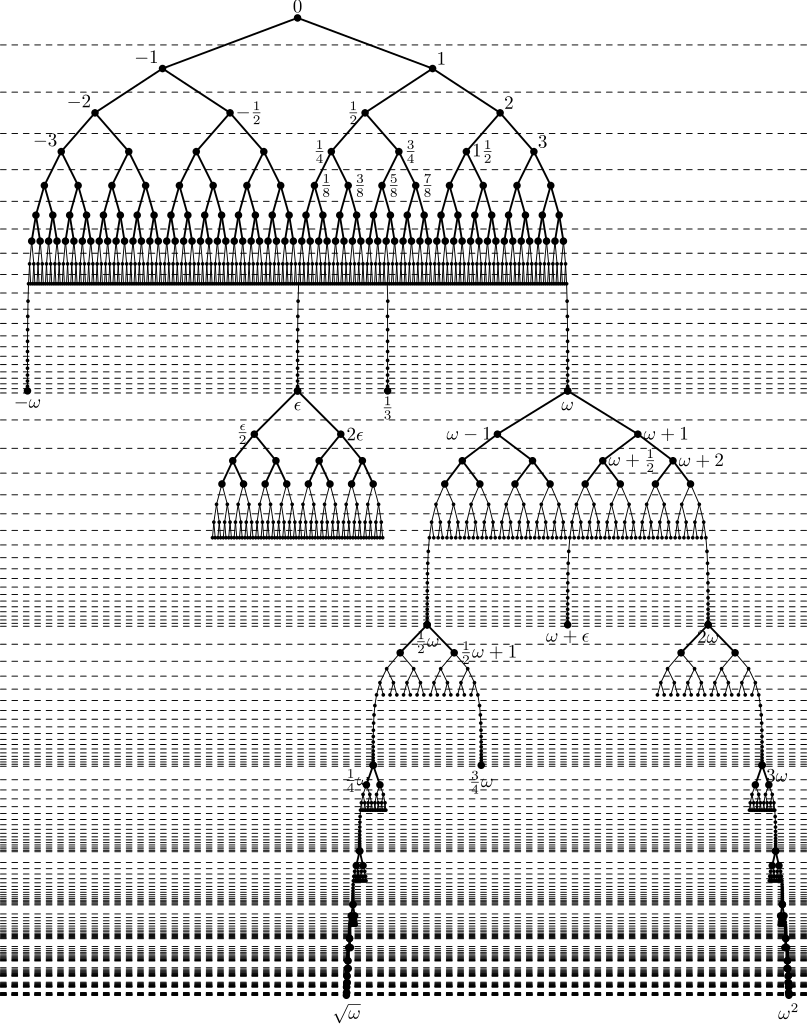
\includegraphics[scale=0.375,natwidth=811,natheight=1024]{CGT/811px-Surreal_number_tree.svg.png}
\end{center}

如上图建立超现实数树. 则有对于所有超现实数 $S=\{\mathcal L|\mathcal R\}$, 满足 $S=\{\max\mathcal L|\min\mathcal R\}$ $\max\mathcal L<S<\min\mathcal R$ 内, 且在上图中为最靠近根的那个节点对应的数.

迄今定义的超现实数已经可以用于解决不平等博弈问题, 其余定义均略去. 对于一个游戏, 可以将每个局面映射到一个扩展超现实数上, 所谓扩展, 是没有要求 $\mathcal L$ 中的所有元素均小于 $\mathcal R$ 中元素, 则可能会产生这种元素 $\{0|0\}$, 该元素不等于 0, 但是几乎等价于 0, 记作 $0\parallel\{0|0\}$.

称两个玩家分别为 L 和 R, 以如下方式递归地将所有局面映射为超现实数: 设 $\mathcal L$ 为玩家 L 可以一步达到的局面对应的超现实数集合, $\mathcal R$ 为玩家 R 可以一步到达的局面对应的超现实数集合, 则当前局面对应的超现实数为 $\{\mathcal L|\mathcal R\}$.

多个子局面对应的超现实数可以直接相加. 设某个局面为 $G$, 则胜败条件为:

\begin{itemize}
  \item $G>0$ 则 L 必胜.
  \item $G<0$ 则 R 必胜.
  \item $G\parallel0$ 则先手必胜.
  \item $G=0$ 则后手必胜.
\end{itemize}

\subsubsection{Blue-Red Hackenbush 游戏}
和 Hackenbush 游戏相比 Blue-Red Hackenbush 的不同点就是为每条边染上了红蓝两种颜色, 两个玩家分别只能删去属于自己的颜色的边. 通常来说由于树/图的状态难以保存转移, 因此只考虑链上的 Blue-Red Hackenbush.

下述代码中, 假设为 \lstinline{'L'} 的边为 L 玩家拥有的链边, 则返回值即为该链对应的超现实数.

\lstinputlisting{CGT/surreal.hh}

\subsubsection{Cutcake 游戏}
一块 $n\times m$ 的巧克力沿沟壑纵横切开, L 玩家只能横切, R 玩家只能纵切. 两人一刀会将一块巧克力切成两部分, 下一位切的只能从被切开的小块中选择进行横纵切. 不能切就算败.

本题状态对应的超现实数可以从 $n,m$ 简单求出, 直接给出求超现实数的代码.

\lstinputlisting{CGT/cutcake.hh}
 % 组合博弈论 Combinatorial Game Theory
\clearpage
\section{数列}
\subsection{二项式系数}
\[\binom nk=\frac{n!}{k!(n-k)!}=\begin{cases}1&\text{for }k=0\\\displaystyle\binom {n-1}k+\binom{n-1}{k-1}&\text{otherwise}\end{cases}\]
\paragraph{生成函数:}
\[\sum_{k=0}^n\binom nkx^k=(1+x)^n\]
\paragraph{性质:}
\begin{itemize}
  \item $\displaystyle\sum_{k=0}^n\binom nk=2^n\qquad\sum_{k=0}^nk\binom nk=n2^{n-1}\qquad\sum_{k=0}^nk^2\binom nk=n(n+1)2^{n-2}$
  \item $\displaystyle\sum_{k=0}^nk^3\binom nk=n^2(n+3)2^{n-3}\qquad\sum_{k=0}^nk^4\binom nk=n(n+1)(n^2+5n-2)2^{n-3}$
  \item Vandermonde 恒等式: $\displaystyle\sum_{k=0}^r\binom mk\binom n{r-k}=\binom{m+n}r$.
    \begin{itemize}
      \item $\displaystyle\sum_{k=0}^{\min\{n,m\}}\binom nk\binom mk=\binom{n+m}{\min\{n,m\}}$
      \begin{itemize}
        \item $\displaystyle\sum_{k=0}^n\binom nk^2=\binom{2n}n$
      \end{itemize}
      \item $\displaystyle\sum_{k=0}^n\binom nk\binom n{k-1}=\binom{2n}{n-1}$
    \end{itemize}
  \item 朱世杰恒等式: $\displaystyle\sum_{k=m}^n\binom kr=\binom{n+1}{r+1}-\binom m{r+1}$
\end{itemize}

关于二项式系数求值的代码在组合排列一节的二项式系数中.

\clearpage
\subsection{自然数等幂和 (Bernoulli 数)}
\[
  \begin{alignedat}{8}
    &\sum_{k=1}^mk^0=&m\\
    &\sum_{k=1}^mk^1=&\frac12m&+&\frac12m^2\\
    &\sum_{k=1}^mk^2=&\frac16m&+&\frac12m^2&+&\frac13m^3\\
    &\sum_{k=1}^mk^3=&&&\frac14m^2&+&\frac12m^3&+&\frac14m^4\\
    &\sum_{k=1}^mk^4=-&\frac1{30}m&&&+&\frac13m^3&+&\frac12m^4&+&\frac15m^5\\
    &\sum_{k=1}^mk^5=&&-&\frac1{12}m^2&&&+&\frac5{12}m^4&+&\frac12m^5&+&\frac16m^6\\
    &\sum_{k=1}^mk^6=&\frac1{42}m&&&-&\frac16m^3&&&+&\frac12m^5&+&\frac12m^6&+&\frac17m^7\\
  \end{alignedat}
\]
设 $\displaystyle\sum_{k=1}^mk^n=\sum_{k=1}^{n+1}b(n,k)m^k$, 有递推式
\[
  b(n,k)=\begin{cases}
    1&\text{for }n=0\land k=1\\
    \displaystyle\frac nkb(n-1,k-1)&\text{for }n>0\land k>1\\
    \displaystyle1-\sum_{k=2}^nb(n,k)&\text{for }n>0\land k=1\\
  \end{cases}
\]
Bernoulli 数即为 $b_n=b(n,1)$.

\begin{lstlisting}[language=Python]
#!/usr/bin/env python3
from fractions import Fraction


def main():
    b = [[0] * 101 for n in range(100)]
    for n in range(10):  # 0 ~ 9
        for k in range(2, n + 2):
            b[n][k] = Fraction(n, k) * b[n - 1][k - 1]
        b[n][1] = 1 - sum(b[n])


if __name__ == '__main__':
    main()
\end{lstlisting}

\clearpage
\subsection{Catalan 数}
\[
  C_n=\frac{2n!}{n!(n+1)!}=\begin{cases}
    1&\text{for }n=0\\
    \displaystyle\frac{2(2n-1)}{n+1}C_{n-1}&\text{otherwise}
  \end{cases}
\]
\paragraph{生成函数:}
\[\sum_{k=0}^\infty C_kx=\frac2{1+\sqrt{1-4x}}\]
\paragraph{含义:}
\begin{itemize}
  \item $C_n$ 表示 $\{1,2,3,\ldots,n\}$ 依序进出栈的置换个数, 下述变种均为等价表述.
  \item $C_n$ 表示长度为 $n$ 的所有合法括号序列.
  \item $C_n$ 表示 $n$ 个节点构成的不同构二叉树个数, 下图月牙为空的情况.
  \item $C_n$ 表示 $2n+1$ 个节点构成的不同构非叶节点满孩子的二叉树个数, 下图月牙为叶子的情况.
    \begin{center}
      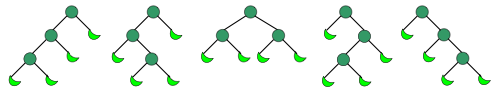
\includegraphics[scale=.5]{SEQ/Catalan_number_binary_tree_example.png}
    \end{center}
  \item $C_n$ 表示在 $n^2$ 格点中不越过对角线的单调路径个数.
    \begin{center}
      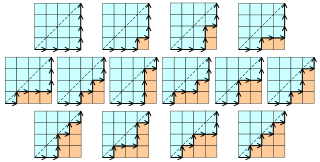
\includegraphics[scale=.5,natwidth=320,natheight=162]{SEQ/320px-Catalan_number_4x4_grid_example.svg.png}
    \end{center}
  \item $C_n$ 表示 $n+2$ 边形划分为三角形方案数.
    \begin{center}
      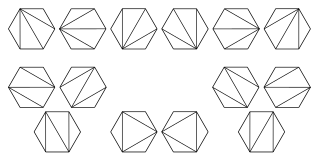
\includegraphics[scale=.5,natwidth=320,natheight=160]{SEQ/320px-Catalan-Hexagons-example.svg.png}
    \end{center}
  \item $C_n$ 表示用 $n$ 个矩形填充一个高 $n$ 的阶梯状图形的方法数.
    \begin{center}
      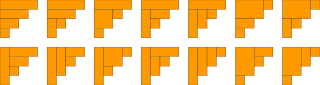
\includegraphics[scale=.5,natwidth=320,natheight=85]{SEQ/320px-Catalan_stairsteps_4.svg.png}
    \end{center}
\end{itemize}

\clearpage
\subsection{Stirling 数}
\[
  \begin{aligned}
    s(n,k)&=(-1)^{n+k}\genfrac[]{0pt}0nk&\genfrac[]{0pt}0nk=&\begin{cases}
      1&\text{for }n=0\land k=0\\
      0&\text{for }n=0\lor k=0\\
      \displaystyle(n-1)\genfrac[]{0pt}0{n-1}k+\genfrac[]{0pt}0{n-1}{k-1}&\text{otherwise}
    \end{cases}\\
    S(n,k)&=\genfrac\{\}{0pt}0nk&\genfrac\{\}{0pt}0nk=&\begin{cases}
      1\qquad\qquad\qquad\qquad\qquad\quad\ \ \text{for }n=0\land k=0\\
      0\qquad\qquad\qquad\qquad\qquad\quad\ \ \text{for }n=0\lor k=0\\k
      \genfrac\{\}{0pt}0{n-1}k+\genfrac\{\}{0pt}0{n-1}{k-1}\qquad\quad\!\!\text{otherwise}
    \end{cases}
  \end{aligned}
\]
\paragraph{生成函数:}
\[\sum_{k=0}^ns(n,k)x^k=x^{\underline n}\qquad\sum_{k=0}^nS(n,k)x^{\underline n}=x^n\]
\paragraph{含义:}
\begin{itemize}
  \item $\genfrac[]{0pt}0nk$ 表示 $n$ 个不同元素的集合划分为 $k$ 个不相交子集, 划分内按环排列的方案数.
  \item $\genfrac\{\}{0pt}0nk$ 表示 $n$ 个不同元素的集合划分为 $k$ 个不相交子集的方案数.
\end{itemize}
\paragraph{性质:}
\begin{itemize}
  \item $\displaystyle\sum_{k=0}^n\genfrac[]{0pt}0nk=n!\qquad\sum_{k=0}^n\genfrac\{\}{0pt}0nk=B_n\qquad\triangleright B_n\text{为 ``Bell 数''}$
  \item $\displaystyle\sum_{k=m}^n\genfrac[]{0pt}0nk\binom km=\genfrac[]{0pt}0{n+1}{m+1}\qquad\sum_{k=m}^n\binom nk\genfrac\{\}{0pt}0km=\genfrac\{\}{0pt}0{n+1}{m+1}$
\end{itemize}
\subsection{Bell 数}
\[
  B_{n+1}=\begin{cases}
    1&\text{for }n=0\lor n=1\\
    \displaystyle\sum_{k=0}^n\binom nkB_k&\text{otherwise}\\
  \end{cases}
\]
\paragraph{含义:}
\begin{itemize}
  \item $B_n$ 表示将含有 $n$ 个不同元素的集合划分为不相交子集的方案数.
\end{itemize}
\paragraph{性质:}
\begin{itemize}
  \item $B_{p^m+n}\equiv mB_n+B_{n+1}\pmod p\qquad\triangleright p\text{为素数}$
\end{itemize}

\subsection{Fibonacci 数}
\[
  F_n=\frac{\phi^n+\psi^n}{\sqrt5}=\begin{cases}
    0&\text{for }n=0\\
    1&\text{for }n=1\\
    F_{n-1}+F_{n-2}&\text{otherwise}
  \end{cases}
\]
\paragraph{生成函数:}
\[\sum_{k=0}F_kx^k=\frac x{1-x-x^2}\]
\paragraph{性质:}
\begin{itemize}
  \item $\displaystyle\sum_{k=0}^{\lfloor n/2\rfloor}\binom{n-k}k=F_{n+1}$
  \item $\displaystyle\sum_{k=0}^nF_k=F_{n+2}-1$
  \item $\displaystyle\sum_{k=0}^nkF_k=nF_{n+2}-F_{n+3}+2$
  \item $\displaystyle\sum_{k=0}^nF_{2k}=F_{2n+1}-1$
  \item $\displaystyle\sum_{k=0}^nF_{2k+1}=F_{2n+2}$
  \item $\displaystyle\sum_{k=0}^nF_k^2=F_nF_{n+1}$
  \item Vajda 恒等式: $F_{n+i}F_{n+j}-F_nF_{n+i+j}=(-1)^nF_iF_j$
  \begin{itemize}
    \item Catalan 恒等式: $F_n^2-F_{n-k}F_{n+k}=(-1)^{n+k}F_k^2$
    \begin{itemize}
      \item Cassini 恒等式: $F_{n-1}F_{n+1}-F_n^2=(-1)^n$
    \end{itemize}
  \end{itemize}
  \item d'Ocagne 恒等式:
  \begin{itemize}
    \item $F_mF_n+F_{m-1}F_{n-1}=F_{m+n-1}$
    \begin{itemize}
      \item $F_{2n-1}=F_n^2+F_{n-1}^2$
    \end{itemize}
    \item $F_mF_{n+1}+F_{m-1}F_n=F_{m+n}$
    \begin{itemize}
      \item $F_{2n}=F_n(F_{n-1}+F_{n+1})$
    \end{itemize}
  \item $\displaystyle F_{an+b}=\sum_{k=0}^a\binom akF_{b-k}F_n^kF_{n+1}^{a-k}$
  \end{itemize}
  \item $\gcd(F_m,F_n)=F_{\gcd(m,n)}$
\end{itemize}

\clearpage
\subsection{分拆数}
\[
p(n,k)=\begin{cases}
  1&\text{for }k=1\\
  0&\text{for }k=0\lor k>n\\
  p(n-1,k-1)+p(n-k,k)&\text{otherwise}\\
\end{cases}
\]

\paragraph{生成函数:}
\[\sum_{k=0}^np(n,k)x^k=\prod_{k=1}^n\frac1{1-x^k}\]

\paragraph{含义:} $p(n,k)$ 表示将 $n$ 个数字拆成 $k$ 个数字的和有多少种方式.

利用五边形数 $O(n\sqrt n)$ 初始化所有小于等于自然数 $n$ 的数的分拆数前缀和 $\displaystyle\sum_{k=1}^\infty p(n,k)$.

\begin{lstlisting}
template <typename RandomAccessIt> void
initIntPart(RandomAccessIt p, size_t n) {
  using T = typename iterator_traits<RandomAccessIt>::value_type;
  vector<T> q = {0, 1, 2, 5};
  while (q.back() < n)
    q.push_back(3 + q.end()[-2] * 2 - q.end()[-4]);
  *p = 1; fill(p + 1, p + n, 0);
  for (size_t i = 1; i != n; ++i)
    for (size_t j = 1; q[j] <= i; ++j)
      p[i] += (j + 1 & 2 ? p[i - q[j]] : -p[i - q[j]]);
}
\end{lstlisting}

对于上述问题的变形, 问将自然数 $n$ 拆分成恰好 $k$ 个不同的数的和的方案数, 有递归公式:

\[
p'(n,k)=\begin{cases}
  0&\displaystyle\text{for }k=0\lor k>\frac{\sqrt{8n+1}-1}2\\
  1&\text{for }k=1\\
  p'(n-k,k)+p'(n-k,k-1)&\text{otherwise}\\
\end{cases}
\]

显然, 计算单个 $p'$ 复杂度为 $O(n\sqrt n)$, 计算前 $n$ 个自然数的 $p'$ 均摊复杂度也为 $O(n\sqrt n)$.

\subsection{错排数}
\[
  \begin{aligned}
    D_n=&n!\sum_{k=0}^n\frac{(-1)^k}{k!}\\
    =&nD_{n-1}+(-1)^n\\
    =&(n-1)(D_{n-1}+D_{n-1})\\
    =&\left[\frac{n!}{\mathrm e}\right]\qquad\text{for }n>1
  \end{aligned}
\]

\subsection{Farey 数列}
$n$ 阶 Farey 数列是 0 到 1 之间最简分数组成的数列, 每个分数的分母均不大于 $n$.

代码中的 \lstinline{Rational} 类见杂项有理数.

\lstinputlisting{SEQ/farey.hh}

\subsection{调和级数}
\[H_n=\sum_{k=1}^n\frac1k\]

\paragraph{性质:}
\begin{itemize}
  \item $\displaystyle\lim_{n\to\infty}H_n=\ln n+\gamma$, 其中 $\gamma$ 为 Euler–Mascheroni 常数, 有 (IEEE-754 binary128 精度): \[\gamma\approx0.57721566490153286060651209008240243\]
\end{itemize}
 % 数列 Sequences
\clearpage
\section{数论}

\subsection{最大公约数/最小公倍数}
Euclidean 算法: $O(\log\min\{n,m\})$.

Stein 算法: $O(\log\max\{n,m\})$, 乘除取模比加减位移效率低时 Euclidean 算法高效.

\[\operatorname{lcm}(n,m)=\frac{nm}{\gcd(n,m)}\]

\lstinputlisting{NT/gcd-lcm.hh}

\subsection{扩展 Euclidean 算法}

求方程 $nx+my=\gcd(n,m)$ 的解. 当已经求得一个解 $(x_0,y_0)$, 可得解集 \[\left\{\left(x_0+\frac{km}{\gcd(n,m)},y-\frac{kn}{\gcd(n,m)}\right):k\in\mathbb Z\right\}\]

下面代码中函数返回值 \lstinline{get<0>} 为 $\gcd(n,m)$, \lstinline{get<1>} 和 \lstinline{get<2>} 组成上述方程的一个解.

\lstinputlisting{NT/exgcd.hh}

\subsection{模逆元}

当 $n\perp m$, 对于方程 $nx\equiv1\pmod m$ 求解 $x$.

问题可以转换为 $nx-mk=1$, 则可用扩展 Euclidean 算法求解.

亦可利用 Fermat-Euler 定理 $n^{\varphi(m)}\equiv1\pmod m$, 得到 $n\cdot n^{\varphi(m)-1}\equiv1\pmod m$, 则 $x\equiv n^{\varphi(m)-1}\pmod m$.

扩展 Euclidean 算法不会有整型溢出. 幂次可能会在乘法过程中溢出.

\lstinputlisting{NT/modinv.hh}

\subsection{原根}
求素数 $p$ 的原根 $g$, $p$ 的原根 $g$ 是幂函数 $a^x\bmod p$ 的最小循环节为 $\varphi(p)$ 的数.

$p$ 的原根存在的充要条件为 $p=2,4,p^k,2p^k$, 其中 $p$ 为奇素数, $e$ 为正整数.

无多项式解, 优化解法是枚举原根, 如果某个数对 $p-1$ 所有因数的幂均不为 1, 则该数为原根.

\lstinputlisting{NT/primitive.hh}

\subsection{离散对数}
求满足 $g^x\equiv y\pmod p$ 的最小的 $x$, 其中 $g\perp p$. Baby-step giant-step 算法, 时空 $O(\sqrt p)$.

\lstinputlisting{NT/bsgs.hh}

若有 $g\not\perp p$, 则需要先将其化为互质:
\lstinputlisting{NT/exbsgs.hh}

\subsection{二次剩余}
求解 $x^2\equiv n\pmod p$, Tonelli Shanks 算法, 时间复杂度 $O(\log^2p)$.
\lstinputlisting{NT/tonelli-shanks.hh}

Cipolla 算法, 时间复杂度 $O(\log p)$. (随机地, 概率为 1/2) 找出一个数 $a$ 使得 $(a^2-n)\bmod p$ 不为二次剩余 (即 Legendre 符号为 $-1$). 设 $\omega^2\equiv a^2-n\pmod p$ 为单位复数建立``复数域''.

根据定义有 $(a+b\omega)(c+d\omega)\equiv (ac+bd\omega^2) + (ad+bc)\omega$, 可以进行乘法, 那么可以直接求得 $x\equiv(a+\omega)^{\mathlarger{\frac{p+1}2}}$.

\subsection{高次剩余}
对于 $x^a\equiv n\pmod p$. 解法是求出 $p$ 的原根 $g$, 有 $x\equiv g^y\pmod p$, 因此有 $g^{ay}\equiv n\pmod p$, 问题化为求解离散对数问题.

\subsection{中国剩余定理}

对于 $n$ 个同余方程组 $x\equiv a_k\pmod{m_k}$, 满足 $m_k$ 之间两两互质, 求解 $x$.

设 $\displaystyle M=\prod_{k=1}^nm_k$. 对于每个 $k\in\{1,\dots, n\}$, 设 $\displaystyle M_k=\frac M{m_k}$, $t_k\equiv M_k^{-1}\pmod{m_k}$, 有 \[\displaystyle x\equiv\sum_{k=1}^na_kt_kM_k\pmod M\]

\lstinputlisting{NT/crt.hh}

当 $m_k$ 之间不两两互质时, 需要扩展中国剩余定理.

\lstinputlisting{NT/excrt.hh}

\subsection{素性测试}
Miller Rabin 算法, 下述代码在 \lstinline{uint64_t} 内正确, 复杂度 $O(13\log n)$. 注意可能需要 \lstinline{uint128_t}.
\lstinputlisting{NT/is-prime.hh}

\subsection{Euler 线性筛}
$O(n)$ 找出 $1,\dots,n-1$ 数中的素数, 求解积性函数以及一部分特殊数论函数对于取值为 $1,\dots,n-1$ 的函数值.

下面代码中 \lstinline{mu} 为 Möbius 函数 $\mu$, \lstinline{phi} 为 Euler 函数 $\varphi$, \lstinline{sigma} 和 \lstinline{k} 为除数函数 $\displaystyle\sigma_k(n)=\sum_{d\mid n}d^k$.

注意每个合数都只会被其最小的素因子筛去. 因此求除数函数 $\sigma$ 时为了处理当前筛到的合数为某个素数倍数的情况, 另外维护 \lstinline{facpow} 数组. \lstinline{facpow[n]} 表示 $n$ 的最小的素因子组成的积, 这样就又将问题化为了两个子问题: 求函数关于某个素数幂次的值, 然后再合并该函数幂次和另一个和其互素的数的函数值.

对于数论函数使用 Euler 筛预处理预处理, 考虑三种情况:

\begin{enumerate}
  \item 参数为素数, 此时该数论函数应当有简单的函数表达.
  \item 参数为合数, 且当前筛到的素数不为其因子, 此时即为两个互素的数合并求函数值.
  \item 参数为合数, 且当前筛到的素数为其因子, 此时可以利用 \lstinline{facpow} 数组辅助求值.
\end{enumerate}

\lstinputlisting{NT/euler-sieve.hh}

\subsection{Euler 函数}
$\varphi(n)$ 是小于等于 $n$ 的整数中和 $n$ 互质的数个数. 可以用 Euler 线性筛预处理.
\[\varphi(n)=n\prod_{p\,\text{为}\,n\,\text{素因子}}\left(1-\frac1p\right)\]
\paragraph{性质:}
\begin{itemize}
  \item $\displaystyle\sum_{d\mid n}\varphi(d)=n$
  \item $a\mid b\implies\varphi(a)\mid\varphi(b)$
  \item $n\mid\varphi(a^n-1)\qquad\text{for }a,n>1$
  \item $\displaystyle\varphi(nm)=\varphi(n)\varphi(m)\frac{\varphi(\gcd(n,m))}{\gcd(n,m)}$
  \item $\varphi(n)\varphi(m)=\varphi(\gcd(n,m))\varphi(\operatorname{lcm}(n,m))$
  \item $\displaystyle\frac{\varphi(n)}n=\frac{\varphi(\operatorname{rad}n)}{\operatorname{rad}n}$, $\operatorname{rad}n$ 为 $n$ 所有不同的素因子的一次方的乘积.
  \item $\displaystyle\sum_{d\mid n}\frac{\mu^2(d)}{\varphi(d)}=\frac{\varphi(d)}d$
  \item $\displaystyle\sum_{\substack{1\le k\le n\\k\perp n}}k=\frac12[n=1]+\frac12n\varphi(n)$
  \item Fermat-Euler 定理 $a^{\varphi(n)}\equiv1\pmod n$
  \begin{itemize}
    \item $a^k\equiv a^{k\bmod\varphi(n)+\varphi(n)}\pmod n\qquad\text{for }a\not\perp n$
    \item $a^k\equiv a^{k\bmod\varphi(n)}\pmod n\qquad\qquad\;\!\text{for }a\perp n$
  \end{itemize}
\end{itemize}

\subsection{Möbius 函数}
\[
  \mu(n)=\begin{cases}
    -1&n\text{无平方数因数且素因子个数为奇数}\\
    0&n\text{有平方数因数}\\
    +1&n\text{无平方数因数且素因子个数为偶数}\\
  \end{cases}
\]
可用 Euler 线性筛预处理.

\paragraph{性质:}
\begin{itemize}
  \item $\displaystyle\sum_{d\mid n}\mu(d)=[n=1]$
  \item $\displaystyle\mu^2(n)=\sum_{d^2\mid n}\mu(d)$
\end{itemize}

\subsection{Möbius 反演}

对于数论函数 $\displaystyle f(n)=\sum_{d\mid n}g(d)$, 有 $\displaystyle g(n)=\sum_{d\mid n}\mu\left(\frac nd\right)f(d)$.

\paragraph{结论:}
\begin{itemize}
  \item $\displaystyle[i\perp j]=\sum_{d\mid\gcd(i,j)}\mu(d)$, 参见 Möbius 函数性质.
  \item $\displaystyle\varphi(n)=\sum_{d\mid n}d\mu\left(\frac nd\right)$, 见 Euler 函数性质.
  \item $\displaystyle\sum_{i=1}^n\sum_{j=1}^m[\gcd(i,j)=d]=\sum_{r=1}^{\left\lfloor\min\left\{\mathlarger{\frac nd,\frac md}\right\}\right\rfloor}\mu(r)\left\lfloor\frac n{rd}\right\rfloor\left\lfloor\frac m{rd}\right\rfloor$
  \item $\displaystyle\sum_{i=1}^n\sum_{j=1}^m\gcd(i,j)=\sum_{k=1}^{\min\{n,m\}}\varphi(k)\left\lfloor\frac nk\right\rfloor\left\lfloor\frac mk\right\rfloor$
\end{itemize}

\paragraph{例子:}
\[
  \begin{aligned}
    &\sum_{i=1}^n\sum_{j=1}^m\frac{ij}{\gcd(i,j)}\\
    =&\sum_{d=1}^{\min\{n,m\}}\frac1d\sum_{i=1}^ni\sum_{j=1}^mj[\gcd(i,j)=d]&&\triangleright\text{提取最大公约数}\ d\\
    =&\sum_{d=1}^{\min\{n,m\}}\frac1d\sum_{i=1}^{\left\lfloor\mathlarger{\frac nd}\right\rfloor}di\sum_{j=1}^{\left\lfloor\mathlarger{\frac md}\right\rfloor}dj[i\perp j]&&\triangleright\text{两个求和同除以}\ d\\
    =&\sum_{d=1}^{\min\{n,m\}}d\sum_{i=1}^{\left\lfloor\mathlarger{\frac nd}\right\rfloor}i\sum_{j=1}^{\left\lfloor\mathlarger{\frac md}\right\rfloor}j\sum_{r\mid\gcd(i,j)}\mu(r)&&\triangleright\text{参见上述结论}\\
    =&\sum_{d=1}^{\min\{n,m\}}\sum_{r=1}^{\left\lfloor\min\left\{\mathlarger{\frac nd,\frac md}\right\}\right\rfloor}d\mu(r)\sum_{i=1}^{\left\lfloor\mathlarger{\frac n{rd}}\right\rfloor}ri\sum_{j=1}^{\left\lfloor\mathlarger{\frac m{rd}}\right\rfloor}rj&&\triangleright\text{将}\ r\ \text{提到和}\ d\ \text{一起}\\
    =&\sum_{k=1}^{\min\{n,m\}}\sum_{r\mid k}kr\mu(r)\sum_{i=1}^{\left\lfloor\mathlarger{\frac nk}\right\rfloor}i\sum_{j=1}^{\left\lfloor\mathlarger{\frac mk}\right\rfloor}j&&\triangleright\text{枚举}\ k=rd\ \text{和其中一个因子}\\
  \end{aligned}
\]

上例最后, $\displaystyle\sum_{r\mid k}kr\mu(r)$ 为两个积性函数 ($\operatorname{id}^{-1}$ 和 $\mu$) 的 Dirichlet 卷积, 因此也是积性函数, 可以用 Euler 筛预处理. 若 $n,m$ 范围特别大, 可以用杜教筛优化复杂度. 具体参考 ``杜教筛''.

剩下的 $\displaystyle\sum_{i=1}^{\left\lfloor\mathlarger{\frac nk}\right\rfloor}i\sum_{j=1}^{\left\lfloor\mathlarger{\frac mk}\right\rfloor}j$ 为等差数列求和, 可以化为 $\displaystyle\frac14\left\lfloor\frac nk\right\rfloor\left\lfloor\frac mk\right\rfloor\left(\left\lfloor\frac nk\right\rfloor+1\right)\left(\left\lfloor\frac mk\right\rfloor+1\right)$.

该例具体实现参考下一页 ``杜教筛''.

\clearpage
\subsection{杜教筛}
对于积性函数 $f(n)$, 求 $\displaystyle F(n)=\sum_{k=1}^nf(k)$.

找到积性函数 $g(n)$ 使得 $g$ 的前缀和 $\displaystyle G(n)=\sum_{k=1}^ng(k)$ 以及 $f$ 和 $g$ 的 Dirichlet 卷积函数 $\displaystyle h=f*g$ 前缀和 $\displaystyle H(n)=\sum_{k=1}^nh(k)$ 容易计算, 有
\[F(n)=H(n)-\sum_{k=2}^nF\left(\left\lfloor\frac nk\right\rfloor\right)g(k)\]

递归分段求 $F$ 即可, 直接计算 $O(n^\frac34)$, 预处理前 $O(n^\frac23)$ 项时总体复杂度最低, 为 $O(n^\frac23)$.

\paragraph{结论:}
\begin{itemize}
  \item $\displaystyle\mathlarger\Phi(n)=\sum_{k=1}^n\varphi(k)=\frac12n(n+1)-\sum_{k=2}^n\mathlarger\Phi\left(\left\lfloor\frac nk\right\rfloor\right)$
  \item $\displaystyle M(n)=\sum_{k=1}^n\mu(k)=1-\sum_{k=2}^nM\left(\left\lfloor\frac nk\right\rfloor\right)$
\end{itemize}

\paragraph{例子:}

计算函数 $\displaystyle f(n)=\sum_{r\mid k}kr\mu(r)$ 前缀和 $\displaystyle F(n)=\sum_{k=1}^nf(k)$. 容易发现 $g(n)=n$ 和 $f$ 的 Dirichlet 卷积函数 $h(n)=1$, 所以有 $H(n)=n$, $G$ 和 $H$ 均可较为轻松地求得.

\begin{lstlisting}
long G(long n) {
  return n * (n + 1) / 2;
}

long F(long n) {
  static unordered_map<long, long> mem;
  if (n < maxn) return Fn[n];  // Fn 为预处理的前 O(n^2/3) 项 F.
  const auto m = mem.find(n);
  if (m != mem.end()) return m.second;
  long r = n;
  for (long i = 2, j; i <= n; i = j + 1) {
    j = n / (n / i);
    r -= F(n / i) * (G(j) - G(i - 1));
  }
  return mem[n] = r;
}

long solve(long n, long m) {
  long r = 0;
  for (long i = 1, j; i <= min(n, m); i = j + 1) {
    const long ni = n / i, mi = m / i, Sn = G(ni), Sm = G(mi);
    j = min(n / ni, m / mi);
    r += Sn * Sm * (F(j) - F(i - 1));
  }
  return r;
}
\end{lstlisting}

\subsection{洲阁筛 (Min\_25 筛)}

对于积性函数 $f(n)$, 求 $\displaystyle F(n)=\sum_{k=1}^nf(k)$. 洲阁筛要求对于素数 $p$ 和任意整数 $c$, $f(p^c)$ 为 $p$ 的多项式. 洲阁筛比杜教筛更普适, 时间复杂度 $O\left(\frac{n^{3/4}}{\log n}\right)$, 空间复杂度 $O(\sqrt n)$.

考虑函数 $\operatorname{m25}(n,k)$ 表示 Eratosthenes 筛已经筛去 $k$ 个素数之后剩下的数的 $f$ 函数的和:

\[\operatorname{m25}(n,k)=\operatorname{m25}(n,k-1)-f(p_k)[\operatorname{m25}(\lfloor n/p_k\rfloor,k-1)-\operatorname{m25}(p_k-1,k-1)]\]

注意到 $\lfloor n/p\rfloor$ 有 $O(\sqrt n)$ 种取值可以一并处理, $p-1$ 小于 $\sqrt n$ 可以预处理.

\subsection{Jacobi 四平方和定理}
$a^2+b^2+c^2+d^2=n$ 的自然数解的个数, 当 $n$ 为奇数时为 $8\sigma_0(n)$, 当 $n$ 为偶数时为 $24\sigma_0(n)$, 其中 $\sigma_0$ 为除数函数.
 % 数论 Number Theory
\clearpage
\section{线性代数}
\lstinputlisting{LA/matrix.hh}

\subsection{异或线性基}
求一个集合互相异或的最大值, 第 $k$ 小值, 支持动态插入. $k$ 小值从 0 开始计数, 即最小值为第 $k=0$ 小值. $k$ 小值至少取集合中的 1 个数 (否则对于任意集合最小值均为 0).

如无必要, 可以将 \lstinline{span} 和 \lstinline{has0} 去除, 它们仅用于求集合中数字异或得到的 $k$ 小值.

\lstinputlisting{LA/xor-basis.hh}
 % 线性代数 Linear Algebra
\clearpage
\section{组合排列}
\subsection{二项式系数}
$\displaystyle\binom nm$ 无取模可直接线性递推, 复杂度 $O(\min\{m,n-m\})$.

\lstinputlisting{CM/binomial.hh}

对较小的素模数 $p$ 求二项式系数可利用 Lucas 定理降低复杂度至 $O(p\log_p\min\{m,n-m\})$

\lstinputlisting{CM/lucas.hh}

$O(nm)$ 打表预处理.

\lstinputlisting{CM/init-binomial.hh}

若 $n$, $m$ 均较小而 $O(nm)$ 较大 (直接储存结果空间超限), 求 $\displaystyle\binom nm\bmod p$, 可以对阶乘和阶乘逆元打表, 再利用公式 $\displaystyle\binom nm\equiv n![m!]^{-1}[(n-m)!]^{-1}\pmod p$ 可 $O(1)$ 求出二项式系数.

\clearpage
\subsection{球放盒方案数}

下表中, $p$ 函数为分拆数, $\displaystyle\binom nm$ 为二项式系数, $\genfrac\{\}{0pt}0nm$ 为第二类 Stirling 数.

\begin{center}
  \begin{tabular}{cccc}
    \toprule
    $n$ 球   &  $m$ 盒  & 空盒 & 方案数 \\
    \toprule
    完全相同 & 完全相同 &  无  & $\displaystyle p(n,m)$\\
    \midrule
    完全相同 & 完全相同 &  有  & $\displaystyle p(n+m,m)$ \\
    \midrule
    完全相同 & 各不相同 &  无  & $\displaystyle\binom{n-1}{m-1}$ \\
    \midrule
    完全相同 & 各不相同 &  有  & $\displaystyle\binom{n+m-1}{m-1}$ \\
    \midrule
    各不相同 & 完全相同 &  无  & $\displaystyle\genfrac\{\}{0pt}0nm$ \\
    \midrule
    各不相同 & 完全相同 &  有  & $\displaystyle\sum_{k=1}^m\genfrac\{\}{0pt}0nk$ \\
    \midrule
    各不相同 & 各不相同 &  无  & $\displaystyle m!\genfrac\{\}{0pt}0nm$ \\
    \midrule
    各不相同 & 各不相同 &  有  & $\displaystyle m^n$ \\
    \bottomrule
  \end{tabular}
\end{center}
 % 组合数学 Combinatorics Mathematica
%\include{S/S} % 字符串处理 String
%\include{CG/CG} % 计算几何 Computational Geometry
%\include{R/R} % 随机化算法 Randomization
\section{杂项}
\subsection{日期}
Julian 历法 Gregorian 历法互转. 可计算星期, 日期差, 数日前/后的年月日等, 全部 $O(1)$.

月份日期均从 1 开始计数, 无公元 0 年, 4 年一闰, 100 年一平, 400 年一闰.

\lstinputlisting{MISC/date.hh}

\subsection{有理数}
\lstinputlisting{MISC/rational.hh}

\subsection{Josephus 问题}
共 $n$ 人, 每 $m$ 人自杀一人, 问第 $k$ 个自杀的人原编号是多少. 返回值 (人头编号) 和 $k$ 均从 0 开始计数, 即第 1 个自杀者之前还有一个第 0 个自杀者.

\lstinputlisting{MISC/josephus.hh}
 % 杂项 Miscellaneous
\section{Java} \subsection{\lstinline[basicstyle=\mono]{BigInteger}}
\subsubsection{构造}
从整数构造的时候, 可以先考虑包中预定义的几个常量: \lstinline{BigInteger.ZERO}, \lstinline{BigInteger.ONE}, \lstinline{BigInteger.TWO} 和 \lstinline{BigInteger.TEN}. 还可以利用一个静态函数从 \lstinline{long} 构造: \lstinline{BigInteger.valueOf}.

一般来说更习惯于从 \lstinline{String} 构造, 直接构造函数即可. 构造函数有第二个可选参数作为字符串表示的进制基底 (其实是重载实现的).

需要将一个对象转成几个基本类型时使用方法 \lstinline{BigInteger.intValue}, \lstinline{BigInteger.longValue} 和 \lstinline{doubleValue} 等. 转为 \lstinline{String} 时则是世界通用的 \lstinline{BigInteger.toString} 方法, 也可以有一个可选参数作为转换成的进制基底.

\subsubsection{运算}
\lstinline{BigInteger} 是不可变类型, 一切运算均不会修改原对象的值, 只会返回新的值, 运算比较好记, 下面列几个常用的, 按复杂度排序的话:

\begin{center}
  \begin{tabular}{ccc}
    \toprule
    操作 & 函数 & 复杂度 \\
    \toprule
    加法 & \lstinline|add| & $O(n)$ \\
    \midrule
    减法 & \lstinline|subtract| & $O(n)$ \\
    \bottomrule
  \end{tabular}\qquad
  \begin{tabular}{ccc}
    \toprule
    操作 & 函数 & 复杂度 \\
    \toprule
    加法 & \lstinline|add| & $O(n)$ \\
    \midrule
    减法 & \lstinline|subtract| & $O(n)$ \\
    \bottomrule
  \end{tabular}
\end{center}

二进制计数 \lstinline{BigInteger.bitLength}, \lstinline{BigInteger.bitCount}.

二进制运算 \lstinline[language=Java]{BigInteger.and}, \lstinline[language=Java]{BigInteger.or}, \lstinline[language=Java]{BigInteger.not}, \lstinline[language=Java]{BigInteger.xor}, \lstinline[language=Java]{BigInteger.andNot}.

\paragraph{$O(n^{\log_23})$:} \lstinline{BigInteger.multiply} \textit{注: JDK 7 使用朴素 $O(n^2)$ 算法, 8 改用 Karatsuba 算法}.

\paragraph{基于乘法} \lstinline{BigInteger.divide} \textit{注: Knuth 长除法和 Burnikel Ziegler 算法}.

\paragraph{基于除法} \lstinline{BigInteger.gcd}
 % Java
\section{黑魔法}
注意下列操作均有一定危险性, 最好在热身赛先测试一遍哪些指令可用不至于运行时错误.

\subsection{扩展栈大小}
\subsubsection{Linux 运行期转移栈}
\lstinputlisting{BM/stack-linux-amd64.cc}

因为不放心 \lstinline{_Exit} 的一些副作用所以保存了一下旧栈指针用来恢复.

如果不想保存旧栈指针, 应当在 \lstinline{main} 最后 \lstinline{fflush(stdout)}, \lstinline{cout << flush}, 并 \lstinline{_Exit(0)} 才能保证程序正常输出并退出.

\subsubsection{Windows 编译期申请栈}
\lstinputlisting{BM/stack-windows-x86.hh}

\lstinline{reserve} 是指运行时栈总大小, \lstinline{commit} 是指程序开始运行时需要系统分配给栈的物理内存大小, \lstinline{commit} 为可选项. 单位为字节.

过大的 \lstinline{commit} 会导致程序启动时间增加, 但是运行时不需要系统另外为栈分配内存页.

\subsection{\lstinline[basicstyle=\mono]{_Pragma} 编译优化}
\lstinputlisting{BM/pragma-optimize.hh}

似乎老版本的编译器会存在 \lstinline{#pragma} 失效的 bug, 此时可以将 \lstinline{__attribute__((optimize("-O3")))} 和 \lstinline{__attribute__((target("...")))} 放在每个函数声明之前或大括号前, 不过效率不如全局高:

\lstinputlisting{BM/attribute-optimize.hh}

\subsection{编译器内建函数}
%\subsubsection{GNU}
\subsubsection{Find First Set}
\lstinline|int __builtin_ffs{,l,ll}(Integral)|

找到参数二进制中从最低位开始的首个 1 的下标, 下标从 1 开始. 若参数为 0 则返回 0.

\subsubsection{Count Leading Zeros}
\lstinline|int __builtin_clz{,l,ll}(Unsigned)|

计数参数二进制中最高位开始的 0 的个数, 参数为 0 时行为未定义.

即在 $n\neq0$ 的情况下返回 $w-\lceil\log_2(n+1)\rceil$, $w$ 为数据类型位长.

\subsubsection{Count Trailing Zeros}
\lstinline|int __builtin_ctz{,l,ll}(Unsigned)|

除了参数为 0 的情况, 该函数等价于对应的内建 FFS-1, 当参数为 0 时行为未定义.

\subsubsection{Count Leading Redundant Sign Bits}
\lstinline|int __builtin_clrsb{,l,ll}(Integral)|

计数参数二进制中从最高位开始和符号位相同的二进制位个数.

\subsubsection{Population Count}
\lstinline|int __builtin_popcount{,l,ll}(Unsigned)|

计数参数二进制中所有 1 的个数.

编译开启 \lstinline{#pramga GCC target("popcnt")} 可优化成一个指令.

\subsubsection{Parity}
\lstinline|int __builtin_parity{,l,ll}(Unsigned)|

如果参数二进制中所有 1 的个数为奇数则返回 1, 否则返回 0.

\subsubsection{Power Integer}
\lstinline|Floating __builtin_powi{,f,l}(Floating, int)|

和 \lstinline{pow} 类似, 计算幂次, 第二个参数为 \lstinline{int}. 无精度保证, 速度快.

\subsubsection{Binary Swap}
\lstinline|Integral __builtin_bswap{16,32,64}(Integral)|

逆序二进制每一字节, 单个字节内每一位保持不变.

\subsubsection{RdRand}
\lstinline|unsigned int __builtin_ia32_rdrand{16,32,64}_step(Unsigned *)|

真随机数生成, 写入到参数指向的地址. 需要打开 \lstinline{#pragma GCC target("rdrnd")}.

\subsubsection{整数加减乘溢出检查}

\lstinline|bool __builtin_sadd{,l,ll}_overflow(Integral, Integral, Integral *)|

\lstinline|bool __builtin_uadd{,l,ll}_overflow(Unsigned, Unsigned, Unsigned *)|

\lstinline|bool __builtin_ssub{,l,ll}_overflow(Integral, Integral, Integral *)|

\lstinline|bool __builtin_usub{,l,ll}_overflow(Unsigned, Unsigned, Unsigned *)|

\lstinline|bool __builtin_smul{,l,ll}_overflow(Integral, Integral, Integral *)|

\lstinline|bool __builtin_umul{,l,ll}_overflow(Unsigned, Unsigned, Unsigned *)|

\lstinline|bool __builtin_add_overflow(type1, type2, type3 *)|

\lstinline|bool __builtin_sub_overflow(type1, type2, type3 *)|

\lstinline|bool __builtin_mul_overflow(type1, type2, type3 *)|

\lstinline|bool __builtin_add_overflow_p(type1, type2, type3)|

\lstinline|bool __builtin_sub_overflow_p(type1, type2, type3)|

\lstinline|bool __builtin_mul_overflow_p(type1, type2, type3)|

无未定义行为的整型溢出检查, \lstinline{_p} 版本无视第三个参数, 其它的将计算结果储存到第三个参数指向的地址. 若有溢出则返回 \lstinline{true}, 否则 \lstinline{false}.

\subsubsection{MSVC}
MSVC 的内置函数需要包含 \lstinline{intrin.h}. 由于正式赛中没有 MSVC 因此自成一小节.

\paragraph{Bit Scan Forward:} \lstinline|unsigned char _BitScanForward{,64}(unsigned long *, Unsigned)|

对于第二个参数, 从二进制最低位开始找到并返回第一个 1 的下标, 写入第一个参数指向的地址. 下标从 0 开始, 函数默认返回 1, 若传入参数为 0 则函数返回 0, 参数一指向被填为 0.

\paragraph{Bit Scan Reverse:} \lstinline|unsigned char _BitScanReverse{,64}(unsigned long *, Unsigned)|

对于第二个参数, 从二进制最高位开始找到并返回第一个 1 的下标, 写入第一个参数指向的地址. 下标从 0 开始, 函数默认返回 1, 若传入参数为 0 则函数返回 0, 参数一指向被填为 0.

\paragraph{Leading Zeros Count:}
\lstinline|Unsigned __lzcnt{16,,64}(Unsigned)|

返回参数二进制前导 0 个数.

\paragraph{Population Count}
\lstinline|Unsigned __popcnt{16,,64}(Unsigned)|

返回参数二进制中 1 个数.

\paragraph{128-bit Multiplication}\mbox{}

\lstinline{unsigned __int64 _umul128(unsigned __int64, unsigned __int64, unsigned __int64 *)}

\lstinline{unsigned __int64 _umulh(unsigned __int64, unsigned __int64)}

\lstinline{_umul128} 的前两个参数为乘法运算参数, 函数返回值为乘法结果 128 位整数的低 64 位, 高 64 位被写入第三个参数指向的地址.

\lstinline{_umulh} 的参数为乘法运算参数, 函数返回值乘法结果的高 64 位.

\subsection{编译器扩展}
\paragraph{三目运算符} \lstinline{value ?: otherwise} 等价于 \lstinline{value ? value : otherwise}.
\paragraph{128 位整数类型} \lstinline{__int128} 和 \lstinline{unsigned __int128}.

\paragraph{128 位浮点类型} \lstinline{_Float128}, 字面量后缀为 \lstinline{Q} 或 \lstinline{q}.

\paragraph{十进浮点类型} C 中是 \lstinline|_Decimal{32,64,128}|, C++ 中在头文件 \lstinline{decimal/decimal} 中命名空间 \lstinline{decimal} 中的三个类 \lstinline|decimal{32,64,128}|, 不建议使用该类型, 建议重新 \lstinline{typedef}:

\begin{lstlisting}
typedef float decimal32  [[gnu::mode(SD)]];
typedef float decimal64  [[gnu::mode(DD)]];
typedef float decimal128 [[gnu::mode(TD)]];
\end{lstlisting}

\lstinline{_Decimal32} 字面量后缀为 \lstinline{df}, \lstinline{_Decimal64} 字面量后缀为 \lstinline{dd}, \lstinline{_Decimal128} 字面量后缀为 \lstinline{dl}. 

\paragraph{范围 \lstinline[basicstyle=\mono]{case}}

支持在 \lstinline{switch}-\lstinline{case} 中使用范围语法, 即 \lstinline{case '0' ... '9':} 表示 \lstinline{'0'} 到 \lstinline{'9'} 闭区间.

\clearpage
\subsection{库扩展}
\subsubsection{\lstinline[basicstyle=\mono]{__gnu_cxx::rope}}
需要包含 \lstinline{<ext/rope>}, 基本操作和 \lstinline{std::basic_string} 类似, 采用数据结构 rope 实现.

原型 \lstinline{__gnu_cxx::rope<CharT, Alloc>}, 有 \lstinline{crope} 作为 \lstinline{rope<char>} 的别名.

Rope 的复制构造是 $O(1)$ 的, 而且极省空间, 可以用作低效 (雾) 的可持久化数据结构使用.  由于该结构在 C++11 之前被设计编写, 因此没有一些 C++11 特性, 如没有针对 rope 的 \lstinline{std::hash} 的偏特化.

下面是一些和 \lstinline{std::basic_string} 不同的接口简表:

\begin{center}
  \begin{tabular}{ccc}
    \toprule
    \textbf{接口名} & \textbf{函数} & \textbf{备注} \\
    \toprule
    访存 & \makecell{\lstinline|at|\\\lstinline|operator[]|} & 返回值非引用 \\
    \midrule
    引用访存 & \lstinline|mutable_reference_at| & \\
    \midrule
    首尾元素 & \makecell{\lstinline|front|\\\lstinline|back|} & 返回值非引用 \\
    \midrule
    首尾常迭代器 & \makecell{\lstinline|begin|\\\lstinline|end|} & 逆向迭代器同理 \\
    \midrule
    首尾迭代器 & \makecell{\lstinline|mutable_begin|\\\lstinline|mutable_end|} & 逆向迭代器同理 \\
    \bottomrule
  \end{tabular}
\end{center}

\subsubsection{\lstinline[basicstyle=\mono]{__gnu_pbds::cc_hash_table}, \lstinline[basicstyle=\mono]{__gnu_pbds::gp_hash_table}}

需要包含 \lstinline{<ext/pb_ds/assoc_container.hpp>}. 它们和 \lstinline{std::unordered_map} 和 \lstinline{std::unordered_set} 类似, 区别在于 \lstinline{find} 返回的迭代器类型叫做 \lstinline{point_iterator}.

\lstinline{cc_hash_table} 采用 seperate chaining 处理冲突, 效率比 \lstinline{unordered_map} 稍高.

\lstinline{gp_hash_table} 采用 open addressing 处理冲突, 效率比 \lstinline{cc_hash_table} 稍低.

\lstinputlisting{BM/pbds-hashtable-prototype.hh}

默认情况下填上 \lstinline{Key} 和 \lstinline{Mapped} 就可以作为映射表使用, 如果 \lstinline{Mapped} 填入 \lstinline{__gnu_pbds::null_type} 则可以作为集合使用, 特别旧的编译器则要用 \lstinline{__gnu_pbds::null_mapped_type}.

\subsubsection{\lstinline[basicstyle=\mono]{__gnu_pbds::tree}}
需要包含 \lstinline{<ext/pb_ds/assoc_container.hpp>} 和 \lstinline{<ext/pb_ds/tree_policy.hpp>}, 和 \lstinline{std::map}, \lstinline{std::set} 类似, 区别在于各种元素查找操作返回的迭代器叫 \lstinline{point_iterator}.

\lstinputlisting{BM/pbds-tree-prototype.hh}

默认情况下填入 \lstinline{Key} 和 \lstinline{Mapped} 即可作为映射表使用. 如果 \lstinline{Mapped} 填入 \lstinline{__gnu_pbds::null_type} 则可以作为集合使用, 特别旧的编译器则要用 \lstinline{__gnu_pbds::null_mapped_type}.

其中 \lstinline{Tag} 和 \lstinline{Node_Update} 决定了树的主要行为, 库中内置了一些类, 默认是 \lstinline{rb_tree_tag}.

\begin{center}
  \begin{tabular}{cc}
    \toprule
    \textbf{标签} & \textbf{类型} \\
    \toprule
    \lstinline|rb_tree_tag| & 红黑树 \\
    \midrule
    \lstinline|ov_tree_tag| & Ordered Vector 树 \\
    \midrule
    \lstinline|splay_tree_tag| & 伸展树 \\
    \bottomrule
  \end{tabular}
\end{center}

\lstinline{Node_Update} 则默认有 \lstinline{null_node_update}, 库中还内置一个 \lstinline{tree_order_statistics_node_update}, 作用是统计子树大小, 用这个才可以求第 $k$ 大的元素.

下面是一些和 \lstinline{std::map} 或 \lstinline{std::set} 不同的接口说明:

\begin{center}
  \begin{tabular}{ccl}
    \toprule
    \textbf{接口名} & \textbf{函数} & \multicolumn{1}{c}{\textbf{备注}} \\
    \toprule
    第 $k$ 大元素 & \lstinline|find_by_order| & 接收零开始的 $k$值, 返回迭代器 \\
    \midrule
    元素大小排名 & \lstinline|order_of_key| & 接收数据, 返回从零开始的排名 \\
    \midrule
    拆分树 & \lstinline|split| & 需要接收一个分界值和接受拆分结果的对象 \\
    \midrule
    合并树 & \lstinline|join| & 接收另一个堆, 在参数中的堆会被清空 \\
    \bottomrule
  \end{tabular}
\end{center}

注意只有红黑树有对数时间的 \lstinline{split} 和 \lstinline{merge} 算法. PBDS 扩展并没有为伸展树实现高效的拆分合并算法 (伸展树理论也可以达到对数级别).

\clearpage
\subsubsection{\lstinline[basicstyle=\mono]{__gnu_pbds::priority_queue}}
需要包含 \lstinline{<ext/pb_ds/priority_queue.hpp>}. 和 \lstinline{std::priority_queue} 类似, 但是包含效率更高的实现和船新的接口, 且迭代器也是 \lstinline{point_iterator}.

原型 \lstinline{__gnu_pbds::priority_queue<ValueType, Compare, Tag, Alloc>}, 其中 \lstinline{Tag} 决定了实现优先队列的数据结构, 库中内置了:

\begin{center}
  \begin{tabular}{cc}
    \toprule
    \textbf{标签} & \textbf{类型} \\
    \toprule
    \lstinline|pairing_heap_tag| & 配对堆 \\
    \midrule
    \lstinline|binary_heap_tag| & 二叉堆 \\
    \midrule
    \lstinline|binomial_heap_tag| & 二项堆 \\
    \midrule
    \lstinline|rc_binomial_heap_tag| & RC 二项堆 \\
    \midrule
    \lstinline|thin_heap_tag| & 瘦堆 (Fibonacci 堆) \\
    \bottomrule
  \end{tabular}
\end{center}

性能上来说配对堆是最高的, 而且支持高效元素修改和合并, 适用于 Dijkstra 算法中, 默认模板参数使用的也是这个.

和 \lstinline{std::priority_queue} 不同的接口说明:

\begin{center}
  \begin{tabular}{ccl}
    \toprule
    \textbf{接口名} & \textbf{函数} & \multicolumn{1}{c}{\textbf{备注}} \\
    \toprule
    构造 & & 可从迭代器范围构造 \\
    \midrule
    加入元素 & \lstinline|push| & 会返回迭代器 \\
    \midrule
    擦除元素 & \lstinline|erase| & 需要接收迭代器 \\
    \midrule
    修改元素 & \lstinline|modiry| & 需要接收迭代器和新值 \\
    \midrule
    清空堆 & \lstinline|clear| & \\
    \midrule
    拆分堆 & \lstinline|split| & 需要接收一个条件函数和接受拆分结果的对象 \\
    \midrule
    合并堆 & \lstinline|join| & 接收另一个堆, 在参数中的堆会被清空 \\
    \midrule
    迭代器 & \makecell{\lstinline|begin|\\\lstinline|end|} & 迭代的值不是有序的 \\
    \bottomrule
  \end{tabular}
\end{center}
 % 黑魔法 Black Magic
\section{战术}
\subsection{上机检查}
\begin{itemize}
  \item 机器一秒速度, 能做多少次相加取模?
  \item 栈大小, 可行递归深度, 扩栈代码可用否?
  \item \lstinline{__int128}, \lstinline{__float128} 可用否?
  \item \lstinline{#pragma} 架构优化可行否?
  \item GNU 扩展库 (\lstinline{rope}, \lstinline{pb_ds}) 可用否?
\end{itemize}

\subsection{战前准备}
\begin{itemize}
  \item 确定厕所位置, 不要在赛场找厕所浪费时间.
  \item 薄荷糖, 提神醒脑.
  \item 零食, 充饥, 切忌太多, 不然易困.
  \item 水, 解渴, 切忌太多, 不然尿急.
\end{itemize}

\subsection{战时策略}
\begin{itemize}
  \item 题意一定要经过两个人确认.
  \item 解题思路一定要经过一个队友确认.
  \item 交给队友的信息一定要对准确度负责.
  \item 注意数据大小, 时限, 内存, 是否应当启用读入优化.
  \item 注意 clarification, 读完题目看一遍, 写完题目看一遍.
  \item 复杂的逻辑先在纸上写好, 以防上机越写越乱.
  \item 不要放空自己, 不要慌, 就算到了最后十分钟也要全神贯注.
\end{itemize}
 % 战术 Strategy and Tactics

\end{document}
